\section{Antecedentes}

\begin{tcolorbox}[breakable]

    Los antecedentes tienen que dar el origen que nos lleva a considerar el Problema que pretende ser resuelto por este proyecto. Introduce al mismo de forma algo más detallada que la introducción.  Describe el escenario sobre el cual se desarrollará y mencionará qué se intentó para solucionarlo.

    Aquí puedo usar referencias al gobierno electrónico y las determinaciones del estado boliviano y de otras instituciones que apoyan la idea de este proyecto.

    \begin{enumerate}
        \item Los trámites son importantes para el funcionamiento del estado
        \item Los gobiernos buscan digitalizarse
        \item Los gobiernos e instituciones prefieren software libre
        \item En Bolivia se hizo reglamentos
        \item Se adjudican obras para desarrollar software
        \item Se hizo el sistema SIAI con módulos de trámites
        \item Se hacen muchos desarrollos desde cero
        \item Existen librerías interesantes
        \item Existe funcionalidad común
        \item La reutilización de software es ventajosa
    \end{enumerate}

\end{tcolorbox}

Durante el desarrollo del sistema SIAI (Sistema de Información Ambiental Industrial) del \say{Ministerio de Desarrollo Productivo y Economía Plural} por parte de la empresa \say{2IES},
se pudo identificar ciertas funcionalidades comunes a muchos sistemas de software gubernamentales,
las cuales tienen que ver con los trámites, un proceso común en la administración pública de los gobiernos.

% MARK: Estado
\subsection{El Estado como Sistema Organizativo}

% Por qué hablaremos del estado
Si bien los temas filosóficos, históricos o políticos parecen carecer de importancia en la presente propuesta,
es importante entender el origen de la problemática señalada más adelante a partir de la concepción misma del gobierno y del estado, pues esto nos encaminará a entender su evolución organizativa,
la cual eventualmente da lugar a la cuestión que se trata en este documento.

% Origen del estado
Para explicar el origen de la organización social y su evolución, que derivará posteriormente en la creación del estado, se pueden identificar dos grandes teorías: 
Teoría de la armonía social y teoría del conflicto \cite{vacarofernandezOrigenEstado2000}. 
La primera propone que la sociedad se organiza a sí misma como una expresión de solidaridad basada en una conciencia común, 
mientras que la segunda indica que lo hace por una tendencia a resolver contradicciones y tensiones. 
Para los teóricos de la armonía social, \textquote{el estado aparece como la solución colectiva de necesidades nuevas que surgen a partir de situaciones también nuevas}\cite[3]{vacarofernandezOrigenEstado2000}.

% Definición básica del estado
Para lo que nos atañe, el estado es un fenómeno político que supuso la separación o la salida de lo político del terreno social y 
\textbf{la conversión del individuo en un ciudadano}, cuya relación de pertenencia fundamental será con el estado al margen de cualquier característica particular \cite{gordilloperezPorQueSurge2017}.
Esto implica que el ciudadano tiene en adelante una serie de obligaciones para con el estado al cual pertenece, así como derechos.

% Listado de los componentes del estado
El estado no podría terminar de definirse sin mencionar los componentes o elementos que lo acaban materializando, que son 4 \cite{delarocharadaElementosParaTeoria2019}:

\begin{itemize}
    \item Territorio
    \item Población
    \item Gobierno
    \item Soberanía
\end{itemize}

% MARK: Gobierno
\subsection{Gobierno, Burocracia y Administración Pública}

Dentro de los 4 componentes listados, el gobierno 
(del griego $\kappa \upsilon \beta \varepsilon \rho \nu \acute{\epsilon} \iota \nu$ kybernéin \textquote{pilotar un barco} o \textquote{capitán de un barco}), 
es un sistema orgánico de autoridades a través del cual se expresa el poder del Estado, creando, afirmando y desenvolviendo el orden jurídico \cite{fernandezruizDerechoParlamentario2023}. 
Es por tanto un actor que materializa el poder del estado hacia la población.

% Necesidad de practicar la burocracia
Este sistema requiere casi siempre la práctica de la burocracia 
(término acuñado en el siglo 18 por el filósofo Francés Vincent de Gournay, derivando del francés \textit{bureau} y \textit{cratie} que significan \say{Escritorio para escribir} y \say{Gobierno} respectivamente \cite{rockmanBureaucracyStructureProcesses2024}), 
que según Weber es técnicamente la forma más avanzada de ejercer o empuñar el poder por aquellos que lo controlan \cite[114]{watersWeberRationalismModern2015} (el gobierno). 

% Qué es burocracia
El mismo sociólogo alemán, Max Weber, define burocracia como una forma racional de organización que en su opinión es la forma más pura de sistema legal de autoridad. 
La burocracia es según él, necesaria y algunas de sus características fundamentales son las jerarquías, la especialización y la definición estricta de reglas y regulaciones \cite{archerDictionaryPublicAdministration2022}. 
Increíblemente y, a pesar de la experiencia popular, la burocracia se supone en principio como una manera racional de organizar de forma eficiente.

% Crítica a la burocracia
Sin embargo, esta forma de organización suele tener como consecuencia en la práctica una connotación negativa, 
ya que implica el consumo de mayores tiempos de ejecución para distintas tareas administrativas, como es el caso del trámite.

% Presentación de la administración pública
Este tipo de organización aplicada de forma transversal en las distintas instituciones del gobierno,
convive con otra figura importante y también transversal, que es la de la administración pública,
que es \textquote{la que tiene la gestión de los asuntos comunes respecto al ciudadano como miembro del estado} \cite{guerreroCharlesJeanBonninSiglo2020}.

% Origen de la administración pública
La concepción de administración pública se remonta a muchos años atrás. 
Por ejemplo, en el año 302 D.C. Claudio Mamertino ya hablaba del término \say{administración de la cosa pública} (\textit{administratione res publicae}) \cite{nixonPraiseLaterRoman1994}. 
Y es que está estrechamente relacionada con el ejercicio de cualquier tipo de gobierno. 
Sin embargo, la aplicación y definición de la misma no estaría clara hasta la llegada de \textbf{Charles-Jean Baptiste Bonnin} (1772-1846), 
el padre de la ciencia de la administración pública moderna.

% El trámite es un mecanismo de contacto del pueblo con el estado mediante la administración
La administración pública pone en contacto directo a la población con el poder político \cite{mostajomachicadoDerechoAdministrativoAdministracion2016} 
y lo hace de forma inmediata a diferencia de algún poder como el legislativo o el judicialo, los cuales se contactan con el ciudadano de forma mediata. 
Aunque las maneras de efectuar este contacto pueden ser varias, la ciencia de la administración pública no aborda exhaustivamente las mismas. 
Sin embargo, desde una perspectiva heurística y basada en la experiencia como ciudadano de un estado, parece evidente que una de las formas más comunes es aquella que se realiza mediante el trámite.

% MARK: Trámite
\subsection{El trámite}

Poco se ha escrito estrictamente sobre los trámites a nivel académico. 
El mismo término parece ser poco universal y tener especial significado en el español de la región. 
En inglés, por ejemplo, no existe una traducción exacta para la palabra trámite. 
Sin embargo, por conocimiento popular se sabe lo que significa. 
Se sabe también lo estrechamente relacionado que está con el gobierno, la burocracia y el manejo de documentos y, 
a pesar de que también se puede usar en otros contextos, la sociedad parece asociarlo casi siempre con lo antes descrito.

La palabra trámite viene del latín \say{\textit{trames}}, \say{\textit{tramitis}}, que para los romanos significaba \say{senda}, \say{camino}, de donde se derivó el sentido actual de \say{vía legal o procedimiento que debe seguir una gestión}\cite{TramiteCastellanoPagina}. 
En inglés no existe una palabra que tenga la traducción exacta de trámite, pero en la literatura de este idioma se usan distintas palabras como \say{\textit{Procedure}}, \say{\textit{Transaction}} o \say{\textit{Paperwork}}. 
También en español se puede referir al mismo como \say{Procedimiento administrativo} o \say{Servicio Público Transaccional}. 
En todas estas definiciones se tiene como común denominador a los términos: Proceso, Camino, Papeleo, Transacción.

% MARK: Trámite Defs.
Al respecto, de acuerdo a una definición que el Gobierno de México indica en uno de sus portales web, se entiende como trámite a:

\begin{displayquote} 
    Cualquier solicitud o entrega de información que las personas físicas o morales del sector privado hacen ante una dependencia u organismo descentralizado, 
    ya sea para cumplir una obligación, obtener un beneficio o servicio o, en general, a fin de que se emita una resolución, así como cualquier documento que dichas personas estén obligadas a conservar \cite{epnQueEsTramite}.
\end{displayquote}

En el mismo portal se hace una clasificación de los trámites, donde se señalan 5 tipos de los mismos:

\begin{enumerate}
    \item De naturaleza obligatoria
    \item De beneficio
    \item De conservación
    \item De procedimiento
    \item De consulta
\end{enumerate}

Según la Real Academia de la Lengua Española, se define como: 
\say{Cada uno de los pasos y diligencias que hay que recorrer en un asunto hasta su conclusión} \parencite{asaleDiccionarioLenguaEspanola}.

Los trámites, también llamados \say{servicios públicos transaccionales}, constituyen además 
el conjunto de requisitos, pasos o acciones a través de los cuales los individuos o las empresas piden o entregan información a una entidad pública, con el fin de obtener un derecho o para cumplir con una obligación \cite[36]{rosethFinTramiteEterno2018}. 
Desde esta definición, se puede agrupar a los trámites en las siguientes cuatro categorías:

\begin{enumerate}
    \item Registros, certificaciones y constancias
    \item Obligaciones
    \item Servicios
    \item Permisos
\end{enumerate}

% MARK: Trámite Probs.
Sin embargo, el proceso del trámite puede llegar a ser muy engorroso y perjudicar a los ciudadanos.
Tal es el caso de \textbf{Domitila Murillo}, quien a causa de un trámite debía trasladarse entre varias ciudades de Bolivia para hacer largas filas y vagar perdida entre una cantidad indefinida de requisitos. 
Cuando finalmente logró recibir su cédula (el motivo del trámite), no le quedaron más que dos semanas antes de fallecer \cite{charoskyQuejaComoEnergia2014}.

El caso de Domitila no es aislado. 
Las distancias, la falta de definición de requerimientos y la burocracia afectan al proceso del trámite. 
El tiempo que demandan suele causar un perjuicio para la población, muchas veces llegando a tardar horas por un simple trámite, como se puede ver en la figura \ref{fig:horastramite}.
En esta figura se puede ver que en Bolivia, por ejemplo, un trámite puede durar alrededor de 11 horas. Esto tiene también un impacto económico sobre la gente. 

\begin{figure}[htbp]
    \centering
    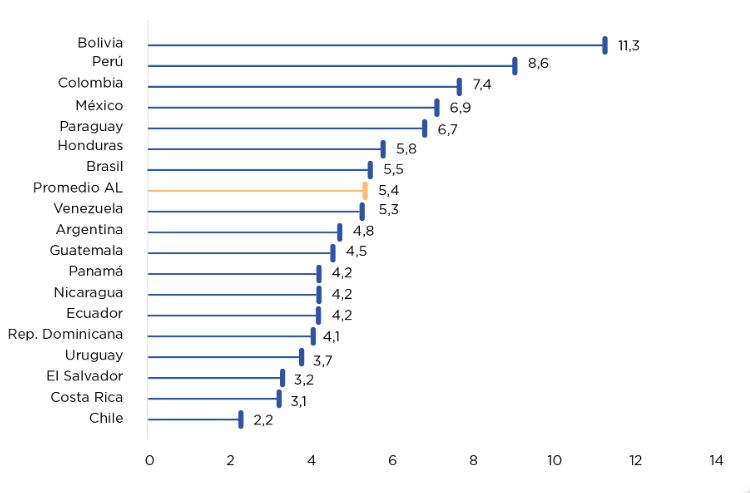
\includegraphics[width=0.7\textwidth]{assets/horastramite}
    \caption{Horas necesarias para completar un trámite, por país}{Fuente: Datos del Latinobarómetro, 2017}
    \label{fig:horastramite}
\end{figure}

Además, como puede verse en la figura \ref{fig:tramites_una_interaccion}, un trámite no suele ser concluido en una sola interacción. 
En Bolivia, por ejemplo, el año 2017 sólo el 38\percentsign ~ de los trámites se resolvieron en un solo encuentro con alguna entidad de la administración pública. 
La situación no es tan diferente en el resto de países de la región, donde en promedio sólo el 50\percentsign de los trámites se lograron en una sola interacción.

\begin{figure}
    \centering
    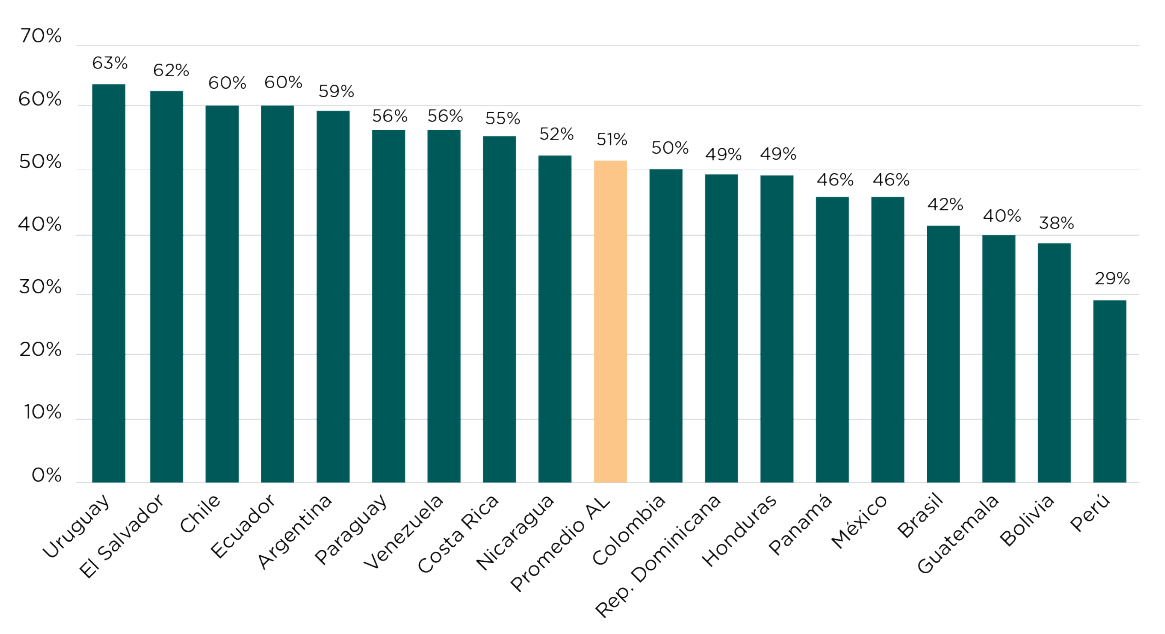
\includegraphics[width=0.7\textwidth]{assets/tramites_una_interaccion}
    \caption{Porcentaje de trámites resueltos en una interacción}{Fuente: Datos del Latinobarómetro, 2017}
    \label{fig:tramites_una_interaccion}
\end{figure}

% Por los problemas se creó el e-government
Aún tomaría más tiempo hablar sobre la corrupción que rodea al proceso del trámite convencional, 
donde algunos funcionarios públicos reciben sobornos de ciudadanos que buscan agilizar algún proceso o recibir algún tipo de trato preferencial.
Esto, entre muchos otros problemas dentro de la administración pública, hizo crecer el interés por la utilización de las tecnologías de la información dentro del gobierno.

% MARK: e-gov
\subsection{\textit{e-government}: Más que una tendencia}

En una entrevista a Carlos Jiménez, responsable mundial de \textit{IEEE e-government}, el mismo señala que 
el gobierno electrónico es una fase para llegar a tener gobiernos inteligentes y abiertos y que 
consiste en implantar la tecnología para mejorar procesos administrativos y permitir la interacción con los ciudadanos \cite{digitalGobiernoInteligenteEntrevista2015}.

% e-gob = uso de TICs
Si bien lo anterior nos puede dar una idea sobre lo que es el Gobierno Electrónico, se debe notar que no existe consenso en su definición y que más de una vez el término se usa de forma indistinta con \say{Gobierno Digital} o incluso algunas veces con \say{Gobierno Inteligente}.
Sin embargo, un factor común es el uso de las \textbf{tecnologías de la información} dentro del gobierno, como veremos a continuación mediante algunas definiciones.

% MARK: e-gov Defs.
Según la secretaría de la función pública del Gobierno de México: 
\textquote{El concepto de Gobierno Electrónico incluye todas aquellas actividades basadas en las modernas tecnologías informáticas, en particular Internet, que el Estado desarrolla 
para aumentar la eficiencia de la gestión pública, mejorar los servicios ofrecidos a los ciudadanos y proveer a las acciones de gobierno de un marco mucho más transparente que el actual} \cite{publicaGobiernoDigitalElectronico}.

Por su lado, la AGETIC, institución del Gobierno de Bolivia, define Gobierno Electrónico como: 
\textquote{la aplicación de las tecnologías de la información y la comunicación (TIC) al funcionamiento del sector público, 
con el objeto de incrementar la eficiencia, la transparencia y la participación ciudadana. 
Engloba la interacción digital entre el estado y los ciudadanos, entre entidades públicas, el Estado y los servidores públicos y, entre el Estado y las empresas, 
contribuyendo al uso intensivo de las TIC} \cite{GobiernoElectronico}.

El Banco Mundial lo define como
\say{El uso de las tecnologías de la información y comunicaciones para mejorar la eficiencia, la efectividad, la transparencia y la rendición de cuentas del gobierno}.

Las Naciones Unidas, por su lado, lo definen como 
\say{La utilización de Internet y la \textit{World Wide Web} para entregar información y servicios del gobierno a los ciudadanos}.

El elemento clave en estas definiciones es la \say{gestión pública por medios digitales}\cite{naserGobiernoElectronicoGestion2011}.

% Ventajas del gobierno electrónico

El Gobierno Electrónico brinda muchos beneficios a la población como 
la eliminación de barreras temporales y espaciales, 
acceso igualitario a la información, colaboración, aumento en la producción de bienes y servicios, 
en suma, brinda mayor calidad de vida a la ciudadanía \cite[16]{naserGobiernoElectronicoGestion2011}.

% No sólo se dirige a los ciudadanos
Los beneficios se crean sobre cuatro actores: Gobierno, Empresas, Ciudadanos y Empleados. Generando cuatro tipos de relaciones:

\begin{enumerate}
    \item G2C: Government to Citizen
    \item G2B: Government to Business
    \item G2E: Government to Employee
    \item G2G: Government to Government
\end{enumerate}

Cada una de estas relaciones (figura \ref{fig:g2all}) pueden implicar la realización de trámites o algún tipo de procedimiento.

\begin{figure}[!htpb]
    \centering
    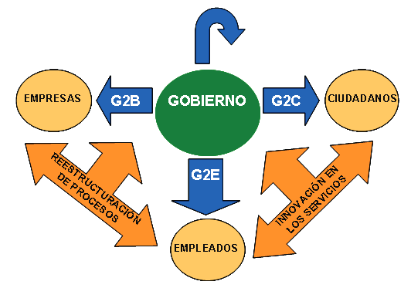
\includegraphics[width=0.7\textwidth]{assets/g2all}
    \caption{Modelo Relacional de Servicios de la Administración Pública}{Fuente: Naser, El Gobierno Electrónico}
    \label{fig:g2all}
\end{figure}

% MARK: e-gob ventjs.
% Es tan ventajoso que gobiernos de todo el mundo lo aplican
Dadas las ventajas que brinda la adopción de las TICs en el área pública, muchos gobiernos del mundo se subieron al tren de la digitalización de sus distintos procesos. 
Al día de hoy se podría decir que ser un gobierno electrónico es más que una simple tendencia y, aunque tras la pandemia del COVID-19 se hizo necesidad, ahora es cada vez más la norma. 
Esto puede verse reflejado en el reporte sobre gobiernos digitales de las Naciones Unidas, 
donde el indicador \textit{EGDI (e-government Development Index)}, que mide la adopción de políticas que favorecen la implementación del gobierno electrónico, 
tuvo un aumento relevante en tan sólo dos años (figura \ref{fig:egdi2020_2022}).

\begin{figure}[!htpb]
    \centering
    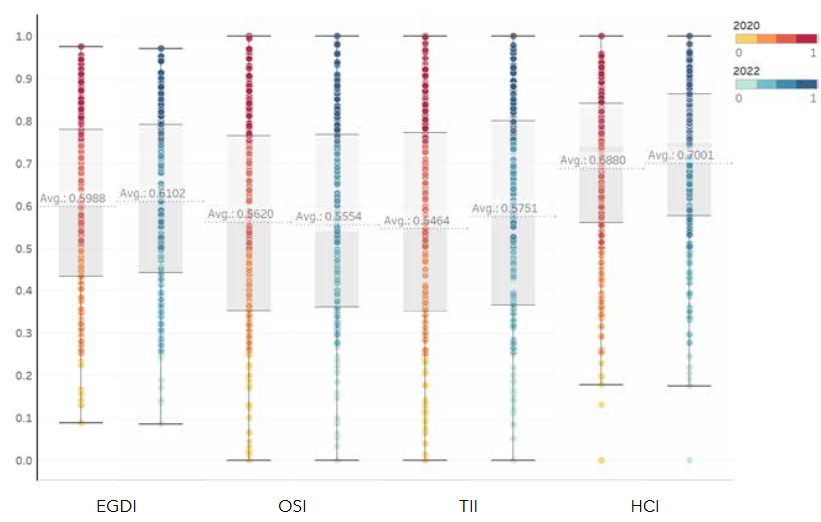
\includegraphics[width=0.7\textwidth]{assets/egdi2020_2022}
    \caption{Valores promedio del EGDI y sus componentes}{Fuente: 2020 and 2022
        United Nations E-Government Surveys}
    \label{fig:egdi2020_2022}
\end{figure}

% MARK: e-gov politics
% Políticas públicas sobre e-government: Caso Bolivia
Para lograr lo anterior cada país implementó políticas públicas y una serie de estrategias que faciliten la adopción y la transición, además de delimitarla de forma correcta.
Tal es el caso de Bolivia con la Ley Nº 164 (\say{Ley General de Telecomunicaciones, Tecnologías de Información y Comunicación}\cite{Ley164Ley2011}), 
los decretos supremos 1793, 3251, 3525 y 3527; resoluciones ministeriales como la Resolución Ministerial Nº 079/20 y distintos planes de implementación \cite{DecretoSupremo17932013}\cite{DecretoSupremoNo2017}\cite{DECRETOSUPREMO35252018}\cite{DecretoSupremoNo2018}\cite{ResolucionMinisterialNo2020}\cite{PLANIMPLEMENTACIONSOFTWARE}.

Esto le brinda características particulares al uso de las TICs dentro del ámbito público, 
las cuales surgen por la naturaleza misma de los gobiernos y sus necesidades específicas como, por ejemplo, la soberanía y la transparencia.

% MARK: FOSS
\subsection{FOSS: Herramientas de libertad}

Cuando Richard Stallman comenzó a trabajar como programador en el Laboratorio de Inteligencia Artificial del MIT el año 1971, 
pasó a formar parte, por primera vez, de una comunidad de \say{\textit{hackers}
\footnote{El término \textit{hacker} es entendido por Stallman como aquel que hace referencia a una persona inteligente y curiosa con espíritu de sagacidad imaginativa y de exploración}}
que \textbf{compartían software} y, sin saberlo porque en aquel entonces la práctica era tan común que no tenía un término propio, eran también una comunidad de \textquote{software libre} \cite{stallmanSoftwareLibrePara}.

% Qué es el software libre de forma resumida
Software libre significa a grandes rasgos que los usuarios tienen la libertad de ejecutar, copiar, distribuir, estudiar, modificar y mejorar el software \cite{QueEsSoftware}.
Por la ambigüedad del término en inglés
\footnote{\textit{free} también puede significar \say{gratis}} 
nació otra forma de referirse a lo mismo, salvo diferencias filosóficas según Stallman\cite{WhyOpenSource}, y que se popularizó bastante: \textbf{\textit{Open Source}}. 
En este documento nos referimos a ellos casi indistintamente y teniendo preferencia por el uso del acrónimo \textbf{FOSS}, \textit{Free and Open Source Software}, que aglutina a ambos.

% Reutilización de software, importancia
En la conferencia sobre ingeniería de software de la OTAN, el año 1968, se hablaba sobre la \say{crisis del software}, 
el problema de construir sistemas de software de gran tamaño, que sean confiables y de costo racional.
En la misma conferencia se vio a la reutilización del software como una posible solución, pero que tenía dificultades para ser aplicada\cite{kruegerSoftwareReuse1992}.
Las distintas libertades descritas del FOSS y la utilización del internet han logrado en los últimos años superar estas dificultades.

Existen muchas ventajas en la reutilización del software, 
como por ejemplo mejoras en productividad al evitar desarrollar la misma funcionalidad o también 
mejoras en calidad al incorporar componentes cuya confiabilidad ha sido ya establecida\cite{selbyEnablingReusebasedSoftware2005}. 
En combinación con la utilización del software libre, se añade una ventaja económica posible e incluso mayor confiabilidad debido a la mayor cantidad de colaboradores posibles.



% FOSS es reutilizable y hay paquetes de software

% Por qué se prefiere FOSS
% Los gobiernos prefieren FOSS
% En Bolivia hay reglamentos para el FOSS
la creación del \textit{Software FOSS} se atribuye a Richard Stallman, conocido
como el padre del código abierto. El mismo creía que todos merecían colaborar
libre y abiertamente con otros utilizando software, por lo que en 1983 presentó
el Proyecto GNU, el cual constituye el primer sistema operativo libre.
Posteriormente en 1985 siguió con la creación de la Free Software Foundation
para apoyar aún más a la comunidad del software libre. A finales de la década de
1990 el reconocimiento generalizado de Linux y el lanzamiento del código fuente
del navegador \textit{Netscape} aumentó el interés y la participación en el
Software libre. La etiqueta de \textit{Open Source} se creó en una sesión
estratégica celebrada el 3 de febrero de 1998 en Palo Alto, California, poco
después de que se publicara el código fuente de \textit{Netscape}. Sin embargo,
el término que actualmente se considera más correcto de usar es el de
\textit{FOSS}, ya que acuña ambas definiciones \textit{(Free and Open Source
    Software)}.

El software libre es principalmente colaborativo y reutilizable, afectando
positivamente a la economía. En un principio, las grandes corporaciones se
negaban a apoyar el desarrollo de \textit{FOSS}. Sin embargo, vista la utilidad
del mismo, hoy en día se prefiere su utilización.

El software que se reutiliza es software de mayor calidad y a menores costos
económicos y temporales. Implica una gran ventaja sobre los desarrollos desde
cero.

% MARK: Digitram
\subsection{El trámite digital}
los trámites por el canal presencial son entre 20 y 42 veces más costosos de prestar que por el canal digital\cite[70]{rosethFinTramiteEterno2018}.
La mala experiencia con los trámites daña la satisfacción ciudadana y la existencia de corrupción en la prestación de servicios reduce la confianza en el gobierno\cite[71]{rosethFinTramiteEterno2018}
Mostrar gráfico 1.35
para aquellos trámites que son indispensables, el canal digital ofrece soluciones a los problemas que existen en el caso de los trámites presenciales: son más rápidos, son más baratos de prestar, y limitan las oportunidades de corrupción \cite[99]{rosethFinTramiteEterno2018}

